\section{Dimensionality Reduction}
The purpose of dimensionality reduction is to:
\begin{itemize}
    \item Avoid curse of dimensionality.
    \item Reduce the amount of time and memory required by data mining algorithms.
    \item Allow data to be more easily visualized.
    \item May help to eliminate irrelevant features or reduce noise.
    \item Recommender systems
\end{itemize}
Some of the techniques used for dimensionality reduction are:
\begin{itemize}
    \item Principle Component Analysis
    \item Singular Value Decomposition
\end{itemize}

This is done by searching for a plane with a lower count of dimensions, which approximately fits the data values.

\subsubsection{Data compression}
By compressing the data, data mining algorithms can be trained faster. Besides, redundant data such as equal measures, but in different units, could be compressed/merged.

\subsubsection{Visualization}
Dimensionality reduction can improve how we display information in a tractable manner for human consumption.
This is important because visually understandable information often helps to develop algorithms.

\section{Singular Value Decomposition (SVD)}
\begin{theo}[SVD]{theo:theo80}
\label{eq:SVD}
\[
A_{[m \cdot n]} = U_{[m \cdot r]} \Sigma_{[r \cdot r]} V_{[n \cdot r]}^T
\]
\end{theo}
Where:
\[
    \begin{aligned}
        & A = \text{Input data matrix} \\
        & \text{I.E m documents, n terms}
        \\
        \\
        & U = \text{Left Singular vectors} \\
        & \text{I.E m documents, r concepts}
        \\
        \\
        & \Sigma = \text{Singular values} \\
        & \text{r - rank of matrix } A
        \\
        \\
        & V = \text{Right Singular vectors} \\
        & \text{I.E n terms, r concepts}
    \end{aligned}
\]

\bigskip
\begin{figure}[H]
\centering
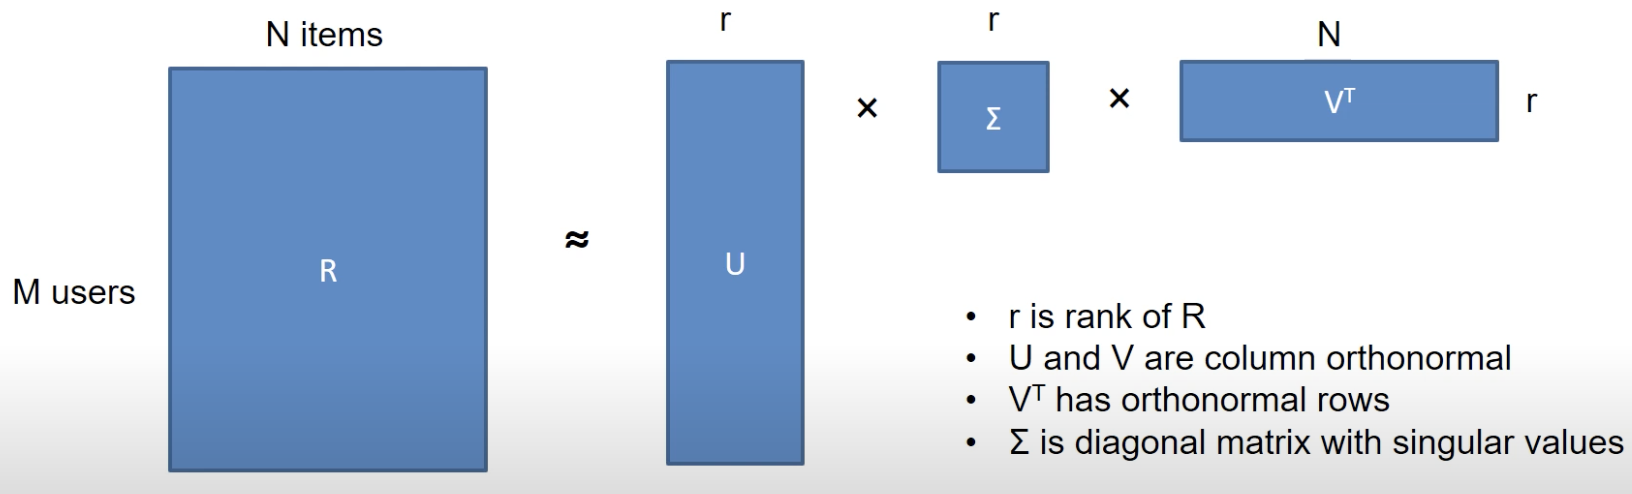
\includegraphics[scale=0.5]{figures/svd.png}
\caption{Single Value Decomposition}
\end{figure}

For information on how to compute the singular value decomposition (with examples), visit: 
\href{http://web.mit.edu/course/other/be.400/OldFiles/www/SVD/Singular_Value_Decomposition.htm}{Singular Value Decomposition (SVD) tutorial}.


\section{Principal Component Analysis (PCA)}
PCA is the most commonly used dimensionality reduction method.

\subsection{Goal}
The goal of the PCA is to find a single line (or plane in higher dimensions) onto which to project the input data.

The line/plane can be found by finding a lower-dimensional surface so the sum of squares onto that surface is minimized.

\subsection{General Case}
\begin{itemize}
    \item Given an $m * n$ matrix, the goal is to find an $m * k$ matrix.
    \item Find a set of vectors which we project the data onto the linear subspace spanned by that set of vectors.
    \item We can define a point in a plane with $k$ dimensional vectors.
\end{itemize}

\subsection{Algorithm}
The PCA Algorithm requires some preprocessing to work properly.
\begin{itemize}
    \item Step 1: Preprocessing
    \begin{itemize}
        \item Mean normalization - Replace each $x_{ji}$ with $x_{ji}$-$\mu_{j}$, subtract the mean from the value, so the mean is re-scaled to be 0.
        \item Feature scaling (dependent on data) - If the features have very different scales, normalize them by changing $x_{ji}$ to $\frac{x_{ij}-\mu_{j}}{s_{j}}$, where $s_{j}$ is some measure of the range, i.e. $max$, $min$, or $standard$ $deviation$.
    \end{itemize}
    \item Step 2: Compute the covariance matrix
    \begin{itemize}
        \item $COV(x, y) = \frac{1}{n-1}\sum_{i=1}^n(x_i-\hat{x})(y_i-\hat{y})$
        \item This results in an $\left[n*n\right]$ matrix.
        \item $x_i$ and $y_i$ are $\left[m*1\right]$ vectors.
    \end{itemize}
    \item Step 3: SVD
    \begin{itemize}
        \item Compute the SVD on the covariance matrix C.
        \item $\left[U, \Sigma, V^T\right] = SVD(C)$
        \item The U matrix is an $\left[n*r\right]$ matrix.
        \item To reduce the system from $n$-dimensions to $k$-dimensions, take the first $k$ vectors from $U$ (The first $k$ columns).
    \end{itemize}
\end{itemize}
\subsection{Transformation}
To change $X$ (which is $n$ dimensional) to $z$ (which is $k$ dimensional):
\begin{enumerate}
    \item Take the first $k$ columns of the $U$ matrix and stack in columns. This gives the $n*k$ matrix $U_{Reduced}$.
    \item Calculate $z$: $z = U_{Reduced}^T * X$
    \item $\left[[k*n]\right]*\left[[n*1]\right]$
    \item This generates a matrix which is $k*1$ per data row.
\end{enumerate}

\subsection{Meassure Quality of PCA}
To meassure how good the implemented PCA is, we can meassure the reconstruction error:
\begin{itemize}
    \item Given the reduced data $U_{Reduced}$ in $K$ dimensions .
    \item $X_{Approx}=U_{Reduce}*Z$ 
\end{itemize}
\begin{equation}
    \frac{\frac{1}{m}\sum_{i=1}^m\norm{x_i-x_i^{approx}}^2}{\frac{1}{m}\sum_{i=1}^m\norm{x_i}^2} \leq 0.01
\end{equation}

\subsection{Choosing the Parameter k}
We want to choose the $k$ value which results in the smallest ratio between the averaged squared projection error with the total variation in the data.
This makes sense, as we want $x_i \approx x_i^{Approx}$ to retain as much information as possible.
